\chapter{Figures and Tables}
\label{sec:first-app}

\section{Figures}

% Todonotes:
\begin{figure}[hbp]
    \centering
    \missingfigure{Insert a picture of the rockfall in Kvam here.}
    \caption[Rockfall]{Initiation area of the Kvam rockfall.}
\end{figure}

% Multiple figures in one
\begin{figure}[htbp]
    \centering
    \begin{subfigure}[t]{0.5\linewidth}
        \centering
        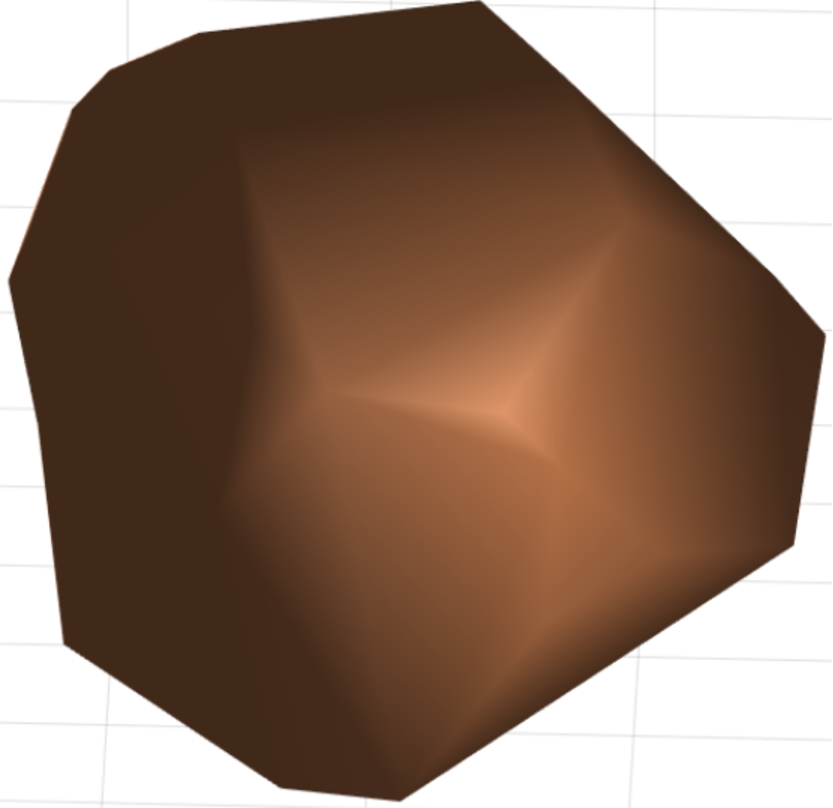
\includegraphics[height = 0.12\textheight]{figures/rock}
        \caption{Rock simulation.}
        \label{fig:rock}
    \end{subfigure}%
    \begin{subfigure}[t]{0.5\linewidth}
        \centering
        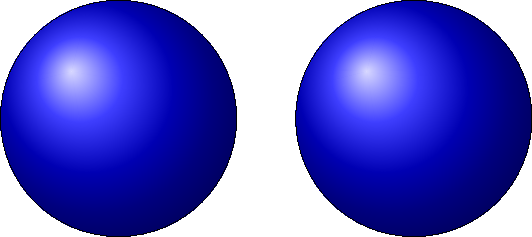
\includegraphics[height = 0.12\textheight]{figures/balls}
        \caption{Balls.}
    \end{subfigure}
    \caption[Subfigures]{A figure with subfigures.}
    \label{fig:rock-and-balls}
\end{figure}

\section{Tables}
\kant[7] % Dummy text

% Math mode for entire column
\begin{table}[htbp]
    \caption[Default friction parameters for different types of terrain]
            {Default friction parameters for different types of terrain \parencite{Bar+11}.}
    \label{tab:friction-parameters}
    \centering
    \begin{tabular}
        {
            @{}
            l
            >{\(}l<{\)} % Specify that each entry in the column starts with \(
            >{\(}l<{\)} % and ends with \)
            >{\(}r<{\)}
            >{\(}l<{\)}
            >{\(}l<{\)}
            @{}
        }
        \toprule
        \textbf{Terrain}
        &
        \boldsymbol{\mu_{\min}}
        &
        \boldsymbol{\mu_{\max}}
        &
        \boldsymbol{\beta_s}
        &
        \boldsymbol{\kappa}
        &
        \boldsymbol{C_v}
        \\
        \midrule
        Extra soft  & 0.2  & 2    &  50 & 1    & 0.9
        \\
        Soft        & 0.25 & 2    & 100 & 1.25 & 0.8
        \\
        Medium soft & 0.3  & 2    & 125 & 1.5  & 0.7
        \\
        Medium      & 0.35 & 2    & 150 & 2    & 0.6
        \\
        Medium hard & 0.4  & 2    & 175 & 2.5  & 0.5
        \\
        Hard        & 0.55 & 2    & 185 & 3    & 0.4
        \\
        Extra hard  & 0.8  & 2    & 200 & 4    & 0.3
        \\
        Snow        & 0.1  & 0.35 & 150 & 2    & 0.7
        \\
        \bottomrule
    \end{tabular}
\end{table}

% Tablefootnote and multirow:
\begin{table}[htbp]
    \centering
    \caption[Dashes]{Proper dash usage.}
    \begin{tabular}{@{}ll@{}}
        \toprule
        \textbf{Correct}
        & 
        \textbf{Incorrect}
        \\
        \midrule
        \( -1 \) 
        & 
        -1
        \\[0.3ex]
        1--10
        &
        1-10
        \\[0.3ex]
        Birch--Swinnerton-Dyer\tablefootnote{It is now easy to tell that Birch and Swinnerton-Dyer are two people.} conjecture
        &
        Birch-Swinnerton-Dyer conjecture
        \\[0.3ex]
        The ball \dash which is blue \dash is round.
        &
        \multirow{ 2}{*}{The ball - which is blue - is round.}
        \\[0.3ex]
        The ball---which is blue---is round. 
        &
        \\
        \bottomrule
    \end{tabular}
\end{table}

% Rotate page
% Columns with fixed width for paragraph-style formatting
\begin{landscape}
    \begin{table}[htbp]
        \centering
        \caption[Long, rotated table]{A long, rotated table.}
        \begin{tabular}
        {
            @{}
            p{0.35\textwidth} % Specify width of column
            p{0.24\textwidth}
            p{0.12\textwidth}
            p{0.35\textwidth}
            p{0.28\textwidth}
            @{}
        }
            \toprule
            \bfseries
            Type of mass movement
            &
            \bfseries
            Location
            &
            \bfseries
            Date
            &
            \bfseries
            Well documented\par
            (media and/or reports)?
            &
            \bfseries
            Hazard mapping?
            \\
            \midrule
            Landslide in rock
            &
            Kvam, Nord-Fron
            &
            11/06/16
            &
            Yes
            &
            Yes (2016, after event)
            \\
            Landslide in rock
            &
            Voss (Fornestræet)
            &
            08/06/16
            &
            Yes
            &
            No
            \\
            Landslide in rock
            &
            Matbjøra
            &
            15/09/16
            &
            Yes
            &
            No
            \\
            Landslide in rock
            &
            Gudvangen
            &
            16/07/16
            &
            Yes
            &
            No
            \\
            \midrule
            Debris flow
            &
            Flåklypa, Lom
            &
            19/05/16
            &
            No
            &
            No
            \\
            Debris flow
            &
            Rindane
            &
            26/11/15
            &
            Yes
            &
            Yes
            \\
            Debris flow
            &
            Skjeldvik, Odda
            &
            26/12/11
            &
            Yes
            &
            No
            \\
            Debris flow
            &
            Beisfjord
            &
            14/07/12
            &
            Yes
            &
            No
            \\
            \midrule
            Debris slide
            &
            Årsetdalen
            &
            09/06/11
            &
            Yes
            &
            Yes (2015)
            \\
            Debris slide
            &
            Borga, Romsdalen
            &
            26/11/15
            &
            Yes
            &
            No
            \\
            Debris slide
            &
            Vatne
            &
            15/11/13
            &
            Yes
            &
            No
            \\
            Debris slide
            &
            Gjerde, Luster
            &
            05/07/15
            &
            Yes
            &
            No
            \\
            Debris slide
            &
            Skredestranda
            &
            15/11/13
            &
            Yes
            &
            No
            \\
            Debris slide
            &
            Berge, Høyanger
            &
            26/12/11
            &
            Yes
            &
            Yes (2014)
            \\
            Debris slide
            &
            Oldedalen
            &
            17/11/13
            &
            Yes
            &
            No
            \\
            \bottomrule
        \end{tabular}
    \end{table}
\end{landscape}